\section{Bias-variance tradeoff}

In practical scenarios, the true model is often unknown, requiring us to select the most appropriate model from a set of options. 
Let's examine the potential solutions for a regression problem:
\begin{itemize}
    \item Hypothesis space: $y(x,\textbf{w})=f(x,\textbf{w})=\sum_{k=0}^{o}x^kw_k$. 
    \item Loss function: $\frac{1}{N}\sum_{(x,t)\in\mathcal{D}}\left(y(x_n,\textbf{w})-t_n\right)^2$ on a dataset $\mathcal{D}$. 
    \item Optimization method: Least Square (LS). 
\end{itemize}
The order $o$ and other parameters, chosen before training, are commonly referred to as hyperparameters.
\begin{figure}[H]
    \centering
    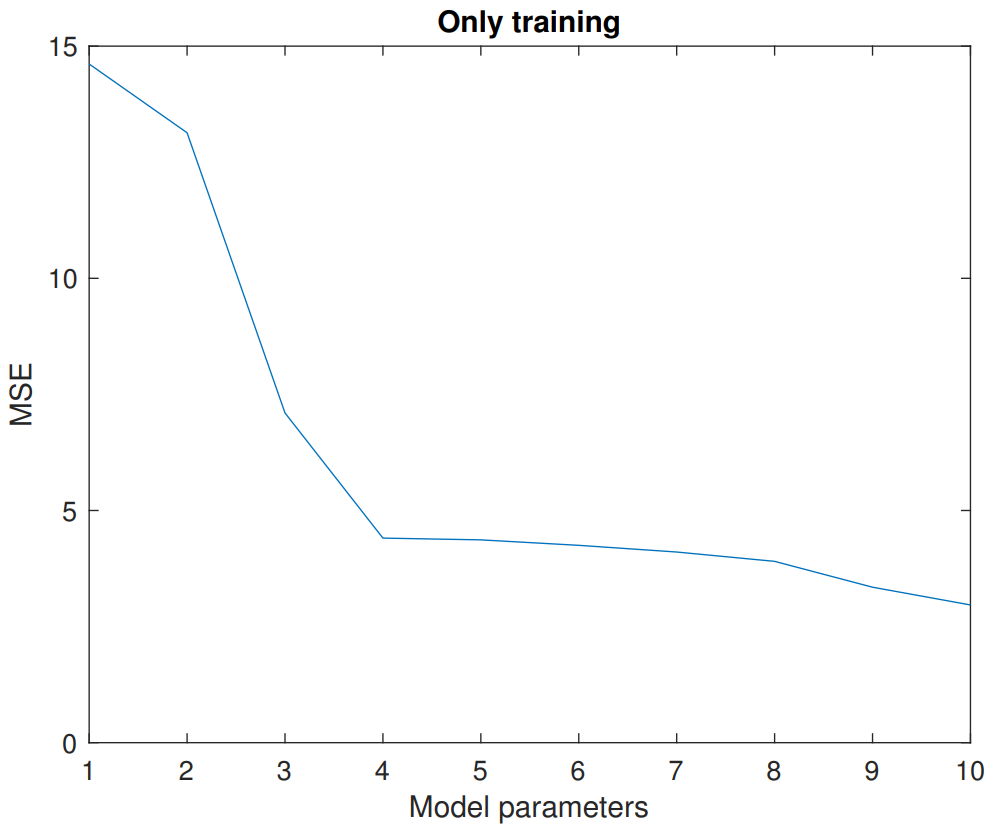
\includegraphics[width=0.5\linewidth]{images/err.png}
    \caption{Training error}
\end{figure}
The error decreases monotonically because the quality of a fixed model $\textbf{w}$ is represented by the expected Mean Squared Error (MSE):
\[\text{MSE}(\textbf{w}):=\mathbb{E}_{\textbf{x},t}\left[\left(y(\textbf{x},\textbf{w})-t\right)^2\right]\]
We train on $\mathcal{D}_{train}$ with $N = \left\lvert \mathcal{D}_{train} \right\rvert $ by minimizing the empirical MSE:
\[\hat{\textbf{w}}\in \argmin_{\textbf{w}\in\mathbb{R}^{o+1}}\hat{\text{MSE}}_{train}(\hat{\textbf{w}}):=\dfrac{1}{N}\sum_{(\textbf{x},t)\in\mathcal{D}_{train}}\left(y(\textbf{x},\textbf{w})-t\right)^2\]
Here: 
\begin{itemize}
    \item $\hat{\textbf{w}}$ is statistically dependent on $\mathcal{D}_{train}$. 
    \item $\hat{\text{MSE}}_{train}(\hat{\textbf{w}})$ isn't a reliable estimate of $\text{MSE}_{train}$ and can't be used for evaluating the performance of $y(\cdot,\textbf{w})$ or for model selection.
\end{itemize}
To address this, we can divide the dataset into two parts:
\begin{figure}[H]
    \centering
    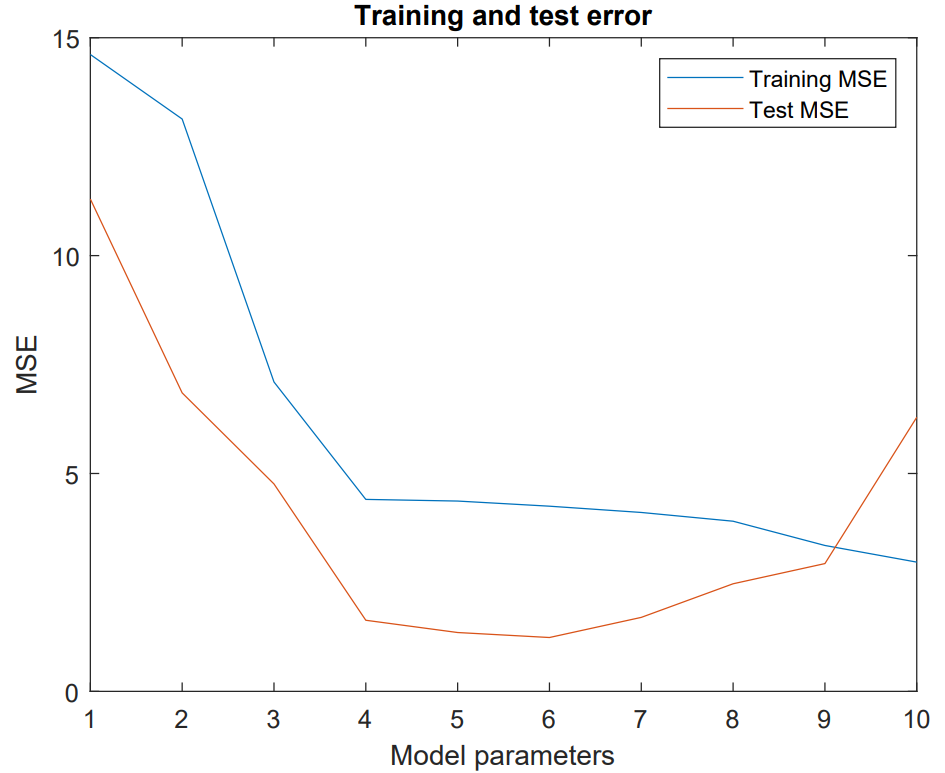
\includegraphics[width=0.5\linewidth]{images/err1.png}
    \caption{Training error with two sets}
\end{figure}
Alternatively, we can employ a test set to evaluate the results, dividing the dataset as follows:
\begin{itemize}
    \item Training set $\mathcal{D}_{train}$: data used for learning model parameters.
    \item Validation set $\mathcal{D}_{vali}$: data used for model selection.
    \item Test set $\mathcal{D}_{test}$: data used for evaluating model performance.
\end{itemize}
Typically, a split of 50\%-25\%-25\% is used for the three sets.
\begin{figure}[H]
    \centering
    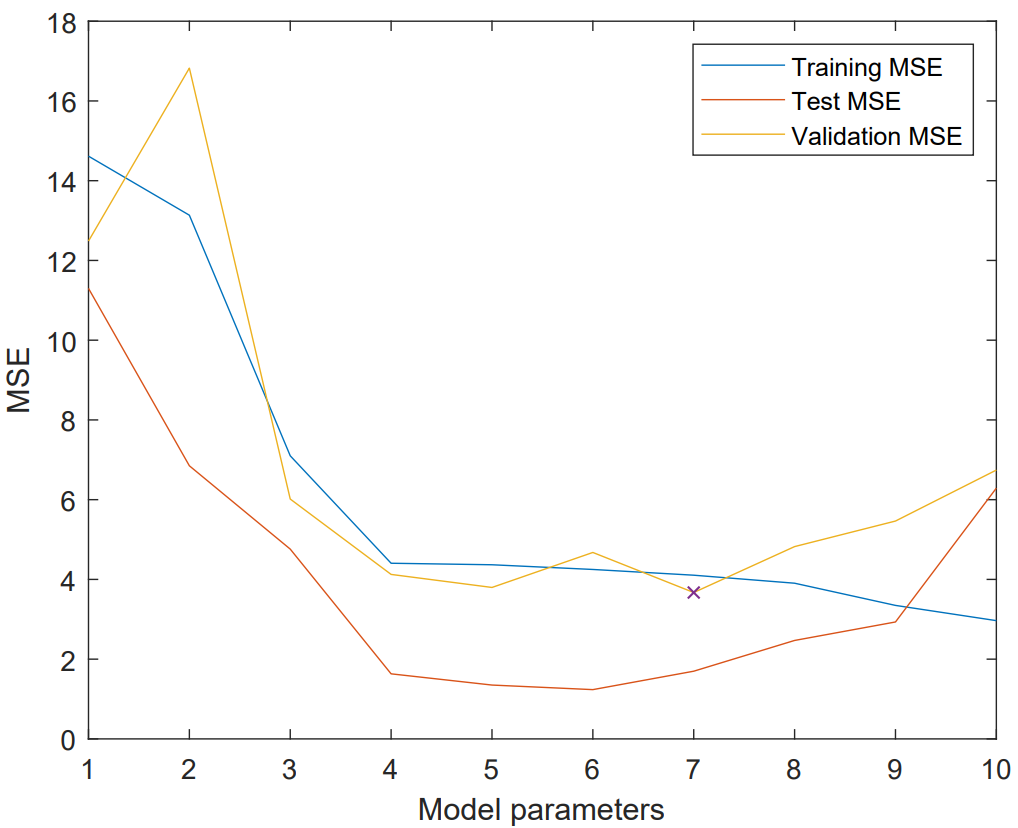
\includegraphics[width=0.5\linewidth]{images/err2.png}
    \caption{Training error with three sets}
\end{figure}